\section{Abstract}
The French 2012-2015 Commission Nationale d'Evaluation reports
\cite{noauthor_reports_2015} emphasize preparation for a transition from \glspl{LWR} to \glspl{SFR}.
This paper uses \Cyclus to explore the feasibility of using \gls{UNF} from other EU nations
for French transition into a \gls{SFR} fleet without additional construction of \glspl{LWR}.
A \Cyclus simulation ran from 1950 to 2160 for EU to track the \gls{UNF} mass
and tails inventory to support
the transition into \glspl{SFR} (66GWe - 110 \glspl{SFR}). The study concludes that France can avoid deployment
of additional \glspl{LWR} by accepting \gls{UNF} from other EU nations.



\section{Introduction}
We used \Cyclus to analyze
the future nuclear inventory in the European Union. \Cyclus is an agent-based extensible
framework for modeling the flow of material through future nuclear cycles \cite{huff_fundamental_2016}.
This paper focuses on the used fuel
inventory in \gls{EU} member states in 2050, and focuses on a potential strategy of used fuel
management.
A major focus of this paper is to determine the extent to which France has an incentive
to receive all the \gls{UNF} from \gls{EU} nations to create \gls{MOX}.
The \gls{MOX} created will fuel French transition to a \gls{SFR} fleet
and allows France to avoid building additional \glspl{LWR}.

Past research focused solely on France typically assumes that additional \glspl{LWR},
namely \glspl{EPR} supply \gls{UNF} to produce \gls{MOX} \cite{carre_overview_2009, martin_symbiotic_2017, freynet_multiobjective_2016}.
Studies exist on implementation of partitioning and transmutation
in a regional (European) context, with \glspl{ADS} and Gen-IV reactors \cite{fazio_study_2013}.
There is little attention paid to reprocessing legacy \gls{UNF} from other
EU nations to produce \gls{MOX} for the newly deployed \glspl{SFR}.
The present work finds that this collaborative strategy can reduce the
need to construct additional \glspl{LWR} in France.

\section{Methodology}

The nuclear history of EU nations are modeled, using the \gls{PRIS} open-source 
database from \gls{IAEA}. That database is imported as a csv file, to populate the simulation
with deployment information, listing the country, reactor unit, type, net capacity (MWe), status,
operator, construction date, first criticality date, first grid date, commercial date, shutdown
date (if applicable), and unit capacity factor for 2013. Then only the \gls{EU} countries are extracted
from the csv file. A python script is written up to generate a \Cyclus input file from the csv file,
which lists the individual reactor units as agents. After running the \Cyclus input file,
another python script analyzes the output file. All the scripts and data used
in this paper are available in \cite{bae_arfc/transition-scenarios:_2017}.
%% Probably a separate repository is needed..?

Two \Cyclus simulations are run for this paper. 
The first simulation calculates
the mass and composition of used fuel and tails \gls{EU} nations accumulate from 1970 to 2050,
as well as the amount of \gls{MOX} that the \gls{UNF} inventory creates.
All EU nations with the exception of France adopts a once-through fuel cycle.
France can reprocess used \gls{UOX} and \gls{MOX} to
produce \gls{MOX} from reprocessed plutonium and depleted uranium (tails).
The simulation assumes infinite \gls{MOX} reprocessing. 

%%% PASSIVE PHRASE WHAT TO DO
After obtaining the \gls{UNF} inventory of all \gls{EU} in 2050, the second
simulation runs where the \gls{UNF} inventory is reprocessed and used
as fuel for the newly deployed \gls{SFR} reactors.
\gls{SFR} reactors in this paper model after the ASTRID reactor.
ASTRID-type \glspl{SFR} make up for the decommissioned capacity
of \glspl{LWR} in France, to remain a constant installed capacity of $66,000$ MWe up to 2160.
It is assumed that ASTRID-type reactors use \gls{MOX} fuel created from 11\% reprocessed plutonium
and 89\% tails and burns the \gls{MOX} fuel to approximately 100 GWdth/t.
The high burnup allows breeding of plutonium.
Eventually, the  \gls{MOX} created from recycled \gls{MOX}
fuels the entire fleet of 110 \glspl{SFR}.


\subsection{Assumptions}
The simulation ran for this paper had the following assumptions:
\begin{itemize}
	\item \gls{SFR} technology is available for deployment in 2040.
	\item Decay is not taken into account.
	\item Reactor construction is always completed on time.
	\item Separated uranium is unused and stockpiled.
	\item \glspl{LWR} have an assumed lifetime of 60 years, unless shut down prematurely.
	\item Newly deployed \glspl{SFR} have a lifetime of 80 years.
	\item Additional assumptions in the \gls{SFR} case include:
	\begin{itemize}
		\item Reprocessing and \gls{MOX} fabrication begins in 2020.
		\item French nuclear capacity remains constant at 66,000 MWe.
		\item Reprocessing and fabrication capacity is unlimited.
	\end{itemize}
\end{itemize}


\subsection{Deployment Timeline}
Projections of future reactor deployment in this simulation is based on assessment of analyses
from references such as \gls{PRIS} for reactors planned for construction \cite{iaea_pris_nodate},
the World Nuclear Association and two other papers for future plans in EU nations
\cite{world_nuclear_association_nuclear_2017, joskow_future_2012, hatch_politics_2015}.
The projections extend to 2050 at the latest. This allows the simulation to take place from
1970 to 2050, the latest foreseeable future. Later sections explain, in detail, the specific plans for each \gls{EU} nation.

Figure \ref{fig:eu_pow} displays the
timeseries of installed capacity in \gls{EU} nations.


\begin{figure}[htbp!]
	\begin{center}
		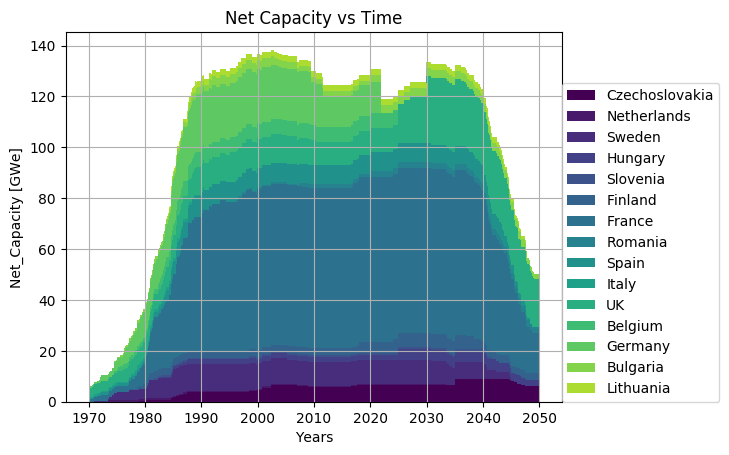
\includegraphics[width=\columnwidth]{./images/eu_future/power_plot.png}
	\end{center}
	\caption{Timeseries of installed nuclear capacity in \gls{EU}.}
	\label{fig:eu_pow}
\end{figure}
\FloatBarrier


\subsection{French \gls{SFR} Deployment Schedule}


Once \glspl{SFR} become available, in 2040,
600-MWe \glspl{SFR} are deployed to make up for the 
decommissioned \gls{LWR} capacities. 
This results in an installed capacity of 66,000 MWe
of \gls{SFR} by 2076, when the last \gls{LWR} decommissions.

\begin{figure}[htbp!]
	\begin{center}
		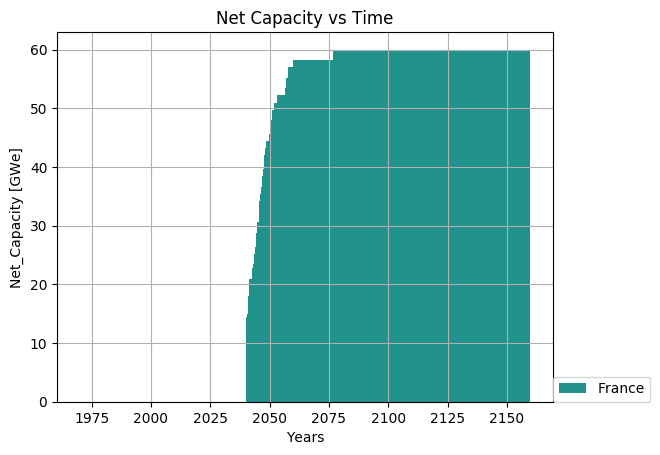
\includegraphics[width=\columnwidth]{./images/french-transition/power_plot.png}
	\end{center}
	\caption{French Transition into an SFR Fleet}
	\label{fig:sfr_num}
\end{figure}
\begin{figure}[htbp!]
	\begin{center}
		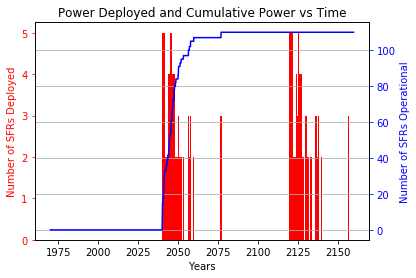
\includegraphics[width=\columnwidth]{./images/french-transition/sfr_deploy.png}
	\end{center}
	\caption{Deployment of French \glspl{SFR} and total installed capacity}
	\label{fig:dep}
\end{figure}
\FloatBarrier


\Cref{fig:sfr_num} and \cref{fig:dep} display
the French transition to \glspl{SFR} over time.
The steep transition from 2040 to 2060 reflects the scheduled
decommissioning of reactors built in the 1975-2000
era of aggressive nuclear growth in France.

\subsection{Material Definitions}
Depletion calculations of the nuclear fuel are recipe-based, such that a fresh 
and used fuel recipe is used for each reactor type.
For the compositions of the fuel, a reference depletion calculation
from ORIGEN is used. The recipe has also been used for
\cite{wilson_adoption_2009}.


\subsection{Scenario Descriptions}
The simulation follows the model fuel cycle
where a `source' provides natural uranium, which is enriched by an 'enrichment'
facility to produce \gls{UOX}, while disposing enrichment waste (tails)
to the 'sink' facility. The enriched \gls{UOX} fuels
the \gls{LWR}s and \gls{UOX} waste is produced. The used fuel
is sent to a pool to cool for 3 years \cite{carre_overview_2009}.
The cooled fuel is then reprocessed to separate plutonium and uranium,
or sent to a repository.
The plutonium mixed with depleted uranium (tails) makes \gls{MOX}.
The reprocessed uranium is unused and stockpiled. Uranium is reprocessed
in order to separate the raffinate (Minor actinides and fission products)
from 'usable' material. Though not utilized in this paper, reprocessed
uranium may substitute depleted uranium for \gls{MOX} production. In this
paper, there was sufficient depleted uranium inventory that using reprocessed
uranium was not considered. However, further in the future where the depleted
uranium inventory drains, reprocessed uranium (or, natural uranium) will need to be utilized. 

